\documentclass[a4paper, 12pt, twoside, final, book, russian, fittopage, cyremdash, openright]{ncc}
\usepackage[a4paper]{geometry}
\geometry{verbose, tmargin=3cm, bmargin=3cm, lmargin=2cm, rmargin=1.5cm, headheight=1cm, headsep=1cm, footskip=1.5cm}
\usepackage[T2A]{fontenc}
\usepackage[utf8]{inputenc}
\usepackage{wrapfig}
\usepackage[section]{placeins}
\usepackage{booktabs}
\usepackage{longtable}
\usepackage{hyperref}
\usepackage{xspace}
\usepackage[headings]{ncchdr}
\usepackage{ncccomma}
\usepackage{desclist}
\usepackage{indentfirst}
\usepackage{upgreek}
\usepackage{marvosym}
\usepackage{multirow}
\usepackage{amsfonts}
\usepackage{enumerate}
\usepackage{rotating}
\usepackage{array}
\usepackage{graphicx}
\usepackage[font=small]{caption}
\usepackage{xfrac}
\usepackage{accents}

\makeindex

\clubpenalty=10000
\widowpenalty=10000

\righthyphenmin=2 % разрешаем переносить два последних символа

\renewcommand{\bfdefault}{b} % плотный жирный

\newcommand{\mps}{~м/с\xspace}
\newcommand{\kph}{~км/ч\xspace}
\newcommand{\otdo}{\,\ensuremath{\div}\,}
\newcommand{\gr}{\ensuremath{\,^\circ}\xspace}
\newcommand{\grC}{\ensuremath{\,^\circ{}C}\xspace}

\graphicspath{{pics/}}

\begin{document}

\author{\LARGE С.\=,Ю.~Зиновьев}
\title{Составление прогноза погоды по местным признакам}
\setyear{....}
\titlefoot{\theyear}
\maketitle


\frontmatter

{\small \tableofcontents}
{\small \listoffigures}
{\small \listoftables}

\openrightorany

\chapter*{Введение}

Погода для мореплавателей \--- прежде всего фактор, определяющий
безопасность плавания. Затем \--- фактор экономический, и, наконец,
как и для всех людей, \--- фактор комфорта, самочувствия и
здоровья. Предсказание погоды, с научной точки зрения, одна из
сложнейших физических задач. Для ее решения существует несколько
методов.

Гидрометеорологическая обстановка \--- это метеорологические и
гидрологические условия\footnote{Содержание, порядок составления и
  оценки прогноза гидрологической обстановки определяются специальными
  документами}, складывающиеся в районах океанов и морей под
воздействием процессов, происходящих в атмосфере и океане и
оказывающих влияние на действия сил, применение оружия и технических
средств Военно-Морского Флота.

Анализ фактической и предсказание (расчет) ожидаемой метеорологической
обстановки необходимы для учета влияния этой обстановки при
планировании операций (действий) и управлении силами флота.

Анализ фактической и предсказание (расчет) ожидаемой метеорологической
обстановки необходимы для учета влияния этой обстановки при
планировании операций (действий) и управлении силами флота.

Под прогнозом метеорологической обстановки (прогнозом погоды)
понимается научно обоснованное предсказание значений метеорологических
элементов и явлений на определенный район и заданный промежуток
времени. Прогноз является конечным результатом анализа атмосферных
процессов, который проводится на основе данных о фактической
метеорологической обстановке и известных физических закономерностей в
развитии атмосферных процессов.

\mainmatter

\chapter{Основные понятия гидрометеорологического обеспечения безопасности плавания}

Воздушный океан находится в постоянном движении.

\textbf{Воздушная масса}\index{воздушная масса} \--- достаточно
большое количество воздуха (высотой от 1~до 10~километров и
горизонтальной протяженностью до нескольких тысяч километров)
сравнительно однородного по своим физическим свойствам и резко
отличного от воздуха соседних районов. В зависимости от
географического расположения очагов их формирования и подстилающей
поверхности воздушные массы получали названия: арктический морской
(континентальный) воздух, воздух умеренных широт морской
(континентальный), тропический морской (континентальный) воздух,
экваториальный воздух.

Вес столба воздуха, распределенного на единице площади, называют
давлением\index{давление}: плотный холодный воздух в приземном слое
создает высокое давление, а более теплый и менее плотный воздух \---
низкое давление.

Разница в давлении между воздушными массами заставляет их двигаться из
области высокого давления к области низкого, но сила трения
подстилающей поверхности, вращение Земли и центробежная сила изменяют
траекторию движения воздушных масс.

\section{Ветер}
\label{sec:wind}

\textbf{Ветры}\index{ветер} \--- это движение потоков воздуха под
действием разности температур и
давлений. \textbf{Штормом}\index{шторм} называется продолжительный
сильный ветер, скорость которого превышает 15\mps{}.
\textbf{Шквалом}\index{шквал} называют внезапное усиление ветра до
штормового с резким изменением направления.
\textbf{Ураганом}\index{ураган} называется буря, когда скорость ветра
превышает 24\mps{}.

\section{Местные ветры}
\label{sec:local_winds}\index{местные ветры}

Под \textbf{местными ветрами} понимают воздушные течения небольшой
горизонтальной протяженности (от нескольких сот метров до десятков
километров), характерные только для определенных географических
районов. Происхождение их различно. Местные ветры могут быть либо
проявлением местных циркуляции (бризы\index{бриз}, горно-долинные
ветры\index{гоно-долинный ветер}), либо они представляют собой
изменения крупномасштабных движений атмосферы под влиянием орографии
местности (фен\index{фен}, бора\index{бора}). Кроме того, в некоторых
районах местными ветрами иногда называют сильные или обладающие
особыми свойствами ветры, которые по существу являются
крупномасштабными течениями. Подробно местные ветры описываются в
лоциях морей.

\section{Катабатические ветры}
\label{sec:catabatic_wind}

Вдоль холодного побережья Гренландии, Антарктиды и в некоторых других
местах наблюдаются так называемые \textbf{катабатические
  ветры}\index{катабатические ветры}, иногда достигающие штормовой
силы. Вследствие охлаждения воздуха он становится более плотным и под
действием силы тяжести стекает по склонам вниз к морю. К семейству
катабатических ветров относится также бора\index{бора}.

\section{Бора}
\label{sec:bora_wind}\index{бора}

\textbf{Бора} \--- это сильный и порывистый ветер, направленный вниз
по горному склону и приносящий в зимнее время значительное
похолодание. Бора наблюдается в местностях, где невысокий горный
хребет граничит с морем. Холодная воздушная масса, встречая на пути
горный хребет, задерживается им; происходит накопление воздуха перед
хребтом. Воздушная масса увеличивает свою вертикальную протяженность
до момента, когда она сравняется с высотой перевала. После этого
холодный воздух через перевал обрушивается в сторону моря в виде
холодного, штормовой силы ветра. Вертикальная мощность боры обычно не
превышает 200\otdo{}500~м, а распространяется она в море на несколько
километров.

В Советском Союзе бора встречается во многих местах, но особой силы
она достигает в зимнее время в районах Новороссийска и Новой Земли,
где скорость ветра в порывах достигает иногда 50\otdo{}60\mps. Бора
наблюдается также в районе Триеста.

Бора возникает как результат переваливания холодных масс воздуха через
горные хребты и их обвал к морю. Бора является типичным ветром для
западных берегов о.~Новой Земли, где ее повторяемость зимой достигает
10\otdo{}11\%. Типичное синоптическое положение, обусловливающее бору,
сводится к наличию над юго-восточной частью Баренцева моря циклона,
перемещающегося на восток, при наличии над Карским морем и севером
Баренцева моря области повышенного давления.

Скорости ветра при боре нередко превышают 40\mps{}, а в порывах могут
достигать 60\mps{}.  Направление ветра при этом обычно восточное. Бора
может наблюдаться в течение нескольких суток и распространяется в море
на расстоянии до 20~миль.

Явления, подобные новоземельской боре, отмечаются также и в других
районах Северного театра. Они наблюдаются у юго-восточных, южных и
юго-западных берегов Гренландии достигая наибольшей повторяемости в
весеннее время года. В прибрежной полосе при боре скорости ветра могут
достигать 60\otdo{}80\mps{}. И распространяться в море на
30\otdo{}40~миль. Направление такого воздушного потока перпендикулярно
береговой черте и направлено в сторону моря.

\section{Смерчи}
\label{sec:tornados}

В условиях большой неустойчивости атмосферной стратификации, когда
образуются мощные кучево-дождевые облака, под ними возникают
вертикальные вихри небольшого диаметра, простирающиеся от поверхности
Земли до нижней границы облаков. Над морем такие вихри называют
\textbf{смерчами}\index{смерч}, а над сушей \---
\textbf{тромбами}\index{тромб}. В Северной Америке тромбы называются
\textbf{торнадо}\index{торнадо}.

Вихрь возникает в передней части грозового облака. У смерчей над морем
диаметр вихря достигает десятков метров, у тромбов над сушей \---
100\otdo{}200~м, а в американских торнадо \--- еще больше. Скорость
вращения воздуха в таком вихре более 100\mps{}. Вращение воздуха
сопровождается поднятием его вверх по спирали. В процессе вращения
вихрь втягивает сверху облако, а снизу \--- воду или пыль с земной
поверхности. Поэтому смерчи и тромбы видны как темные столбы между
облаками и Землей, расширяющиеся сверху и снизу.

Тромбы и смерчи перемещаются вместе с облаком со скоростью
30\otdo{}40\kph{}. Время существования смерчей \--- минуты, тромбов \---
десятки минут, но иногда несколько часов. За это время смерч может над
морем продвинуться на несколько миль, а тромб над сушей \--- на десятки
километров, сметая все на своем пути.

Тромб сопровождается грозой, ливневым дождем, градом. Водяные смерчи
реже связаны с грозами. Тромбы проходят поодиночке, хотя торнадо
изредка наблюдаются по два и более. Смерчи часто возникают целыми
сериями, по несколько вихрей, даже по 20\otdo{}30. Необходимым условием
возникновения вихрей являются высокая температура воздуха и его
большое влагосодержание. Эти условия характерны для атлантического
побережья Северной Америки.

Атмосферное давление в вихре сильно понижено, на десятки
миллибар. Падение давления при прохождении тромба настолько велико и
быстро, что внутреннее давление в зданиях не успевает выровняться с
наружным, поэтому дома, попавшие в сферу действия тромба, иногда
взрываются. Смерчи обладают меньшей разрушительной силой, однако суда
должны избегать встречи со смерчами, что сделать нетрудно, так как они
видны с достаточно большого расстояния.

\section{Тропические ураганы}
\label{sec:hurricans}\index{ураганы!тропические}

В северную часть Атлантического океана в отдельных случаях проникают
\textbf{тропические циклоны}\index{циклоны!тропические}, известные под
названием \textbf{вест-индских ураганов}\index{ураганы!вест-индские},
обладающих огромной разрушительной силой. Подсчитано, что если бы всю
энергию только одного тропического циклона превратить в электрическую,
то ее хватило бы всему человечеству на несколько лет. В среднем за год
в Атлантическом океане наблюдается около 12\otdo{}13 циклонов. Они
характеризуются небольшими размерами, не превышающими в диаметре
100\otdo{}300~миль, низким давлением в центре, достигающим 940~мб,
большими барическими градиентами и скоростями ветра до
40\mps{}. Особенно сильный ветер наблюдается в центральной части
урагана, причем усиливается он внезапно. Таким образом, вест-индские
ураганы представляют собой чрезвычайно опасное явление для
мореплавателей и при их приближении должны быть приняты меры для
расхождения с центром урагана.  Иногда вест-индские ураганы имеют в
диаметре 1000 и более миль. В таких случаях ветер достигает большой
силы только в центральной части урагана диаметром несколько сот
миль. Сильный ветер, связанный с тропическим циклоном, развивает
большую волну, которая распространяется радиально по всем направлениям
и ощущается в виде зыби на больших расстояниях. \textit{Скорость
  распространения зыби больше скорости перемещения циклона, и поэтому
  ее появление в направлении, несовпадающим с направлением дующего
  ветра, может служить одним из важнейших признаков приближения
  урагана}.

\section{Бризы}
\label{sec:breeze}

\textbf{Бризами}\index{бриз} называются реверсивные ветры на берегах
океанов, морей и озер, имеющие суточную периодичность. У поверхности
Земли днем они направлены с моря на сушу \--- морские бризы, а ночью
\--- с суши на море \--- береговые бризы. В низких широтах бризы
образуются в течение всего года, в умеренных и высоких широтах —
обычно в теплое время года.

\begin{figure*}[htb]
   \centering
   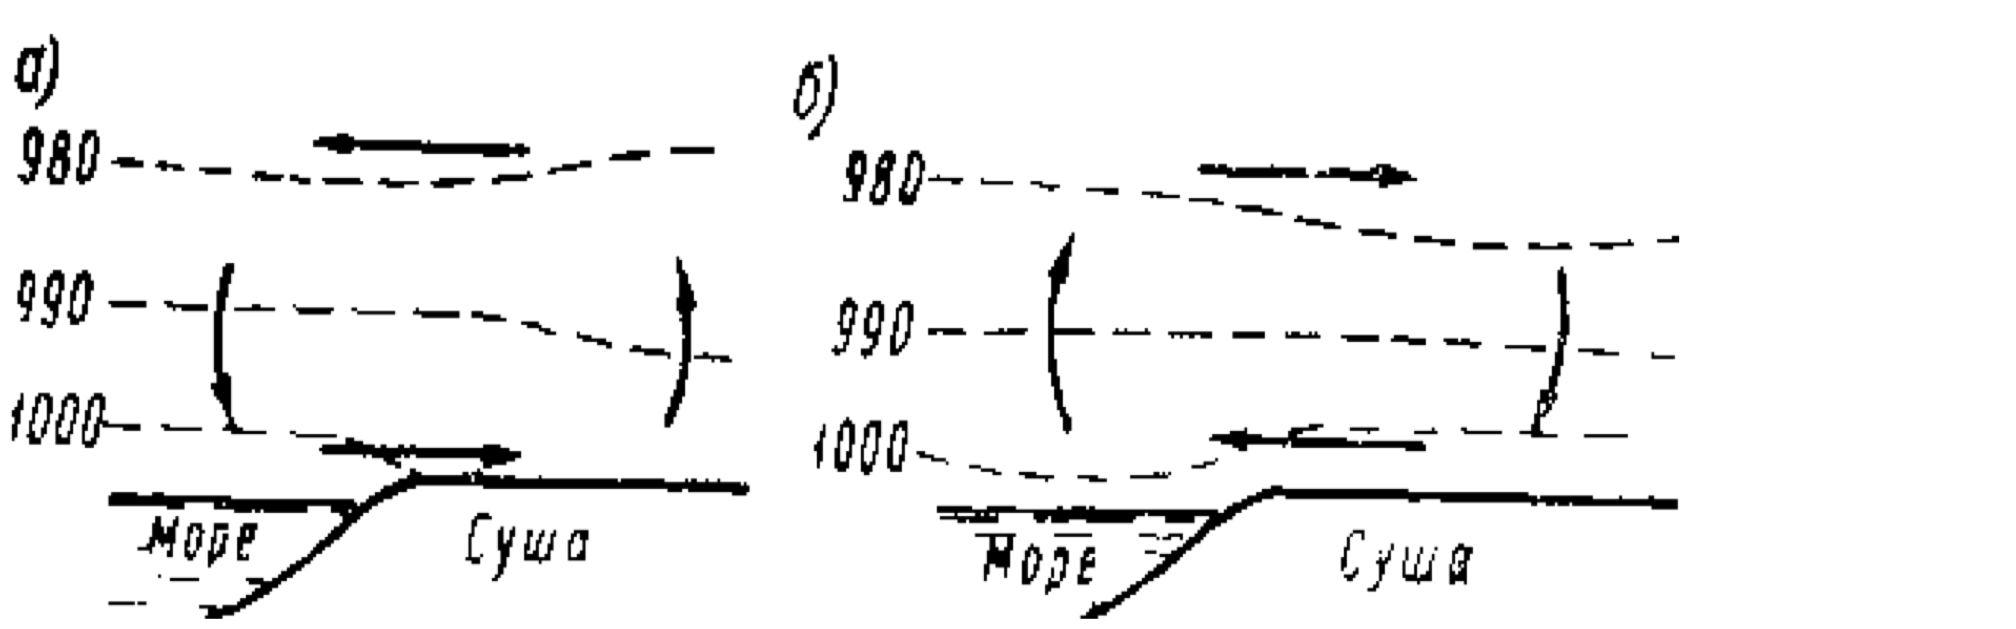
\includegraphics[scale=0.2]{01_breeze.png}
   \caption{Бризы}
   \label{fig:01_breeze}
   \centering{}
   \small
   a)~морской; б)~береговой
\end{figure*}

Причина возникновения бризов \--- неравномерное нагревание и
охлаждение суши и водной поверхности в течение суток. После восхода
Солнца поверхность суши и воздух над ней прогреваются значительно
быстрее, чем море. Так как в теплом воздухе давление с высотой падает
медленнее, чем в холодном, то по мере нагревания воздуха над сушей на
некоторой высоте давление будет выше, чем на той же высоте над
морем. Изобарические поверхности на высотах будут наклонены в сторону
моря, и вследствие этого на высотах начнется отток воздуха с суши на
море (рис.~\ref{fig:01_breeze}). Благодаря увеличению массы воздуха
над морем давление в нижних слоях здесь окажется выше, чем над сушей,
т.е. изобарические поверхности здесь будут наклонены с моря на
сушу. Это приведет к движению воздуха с моря на сушу, т.е. к развитию
ветра, называемого \textbf{морским
  бризом}\index{бриз!морской}. Морской бриз начинается с 8\otdo{}10~ч
утра. Постепенно он усиливается и достигает максимума после полудня,
затем медленно затухает ко времени захода Солнца.

Ночью поверхность суши охлаждается быстрее, чем поверхность моря,
вследствие чего на высотах движение воздуха будет происходить с моря к
суше, а в нижних слоях будет развиваться ветер от суши к морю,
называемый \textbf{береговым бризом}\index{бриз!береговой}. Береговой
бриз начинается после захода Солнца и продолжается до 8\otdo{}9~ч
следующего дня.

Морской бриз обычно сильнее берегового, так как в дневные часы
контраст температур между водной поверхностью и сушей значительно
больше, чем ночью.

Скорость ветра и вертикальные и горизонтальные размеры бризовой
циркуляции весьма разнообразны и изменчивы. Они зависят от суточного
хода температуры воздуха над континентом, а, следовательно, от широты
места, от градиентов давления, а также от рельефа и формы побережья.

Особенно четко бризовая циркуляция проявляется в тропической зоне, где
контрасты температур между поверхностью суши и моря особенно велики.

Так, в тропической зоне морской бриз зарождается на расстоянии
100\otdo{}150~км от берега и проникает на сушу на 80\otdo{}100~км; береговой
бриз распространяется на меньшее расстояние. В умеренных широтах
морской бриз зарождается в 10\otdo{}100~км от берега, и в глубь суши он
распространяется до 30\otdo{}40~км. Скорость ветра при морских бризах в
тропической зоне достигает 5\otdo{}7\mps{}, при береговых \--- 1\otdo{}3\mps{}.

\section{Береговой эффект}
\label{sec:coast_effect}

Рассмотрим случай, когда ветер над морем дует параллельно береговой
черте, идущей, например, в меридиональном направлении. Так как ветер
над сушей отклоняется от изобар на больший угол, чем над морем, то
вдоль западного берега образуется \textbf{зона
  дивергенции}\index{дивергенции зона} (расходимость линий тока), в
которой происходит ослабление ветра, опускание масс воздуха, а
следовательно, устанавливается безоблачная погода. Наоборот, вдоль
восточного берега образуется \textbf{зона
  конвергенции}\index{ковергении зона} (сходимость линий тока) и
соответственно будет происходить усиление ветра, развитие восходящих
движений воздуха, что способствует образованию облачности и выпадению
осадков. Такое изменение силы ветра называется \textbf{береговым
  эффектом}\index{береговой эффект}
(рис.~\ref{fig:02_coast_effect}. Ветер в прибрежной зоне всегда
усиливается, если суша располагается справа от направления линии тока
ветра, и ослабевает, если суша слева. Береговой эффект будет
наблюдаться и в случае, когда ветер дует под острым углом к береговой
черте. Этот эффект усиливается, если берег высокий или гористый.

\begin{figure*}[htb]
   \centering
   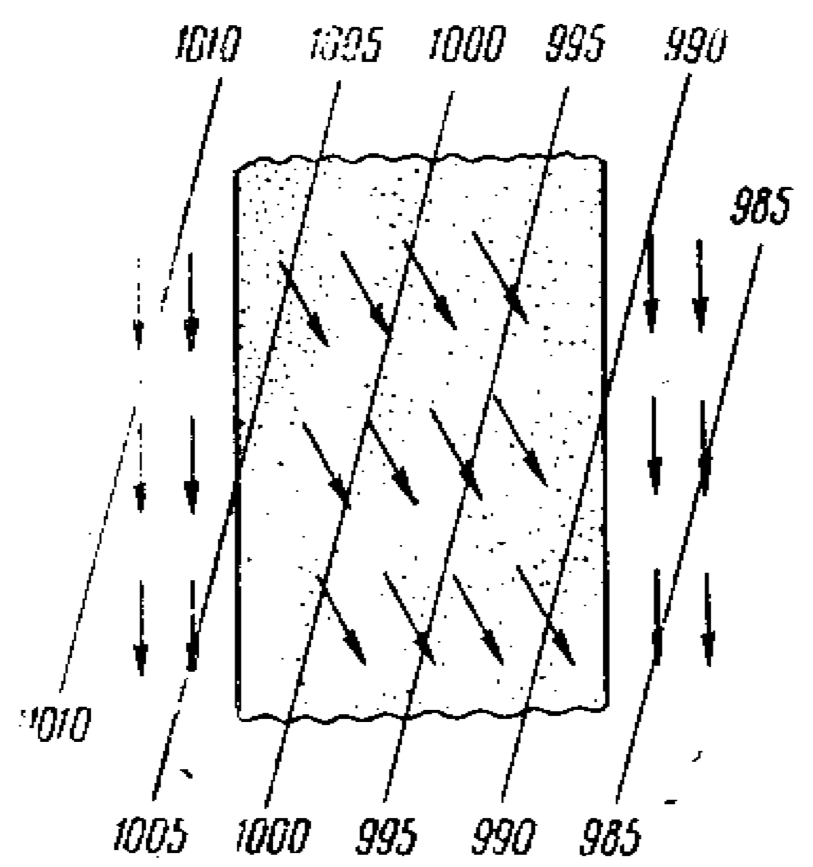
\includegraphics[scale=0.2]{02_coast_effect.png}
   \caption{Береговой эффект}
   \label{fig:02_coast_effect}
\end{figure*}

Всякое препятствие, стоящее на пути воздушного потока, отклоняет его,
и он либо обтекает препятствие с боков, либо перетекает через него
сверху. При горизонтальном обтекании ветер усиливается у мысов,
оконечностей островов и т.п., так как линии тока в таких местах
сближаются. Это усиление ветра называется \textbf{угловым
  эффектом}\index{угловой эффект}. Если мыс или остров остается справа
от направления линии тока, то ветер будет особенно сильным. Примером
является \textbf{бакинский норд}\index{бакинский норд} \--- ветер
северных направлений у Апшеронского полуострова на Каспийском море.

Существенное усиление ветра наблюдается в проливах с высокими
берегами, причем в них преобладают ветры, дующие вдоль пролива.  За
препятствиями скорость ветра уменьшается, и там образуется ветровая
тень. Этим объясняется известный факт, что в заливах, бухтах и фьордах
ветер значительно слабее, чем в открытом море.

\section{Изобары}
\label{sec:isobars}

\textbf{Изобарами}\index{изобары} называются линии, соединяющие на карте точки с равным атмосферным давлением.

\section{Барическое поле}
\label{sec:baric_field}

\textbf{Барическое поле}\index{барическое поле} \--- распределение давлений на каком-либо горизонтальном уровне.

\section{Формы барического рельефа}
\label{sec:baric_relief}

\textbf{Формы барического рельефа}\index{барического рельефа форма}
\--- системы расположения изобар, характеризующие тип падения или
повышения давления. Различают следующие формы барического рельефа:
\textbf{циклон}, \textbf{ложбина}, \textbf{антициклон},
\textbf{отрог}, \textbf{гребень} или \textbf{клин},
\textbf{седловина}.

\section{Барическая тенденция}
\label{sec:baric_tendency}

\textbf{Барическая тенденция}\index{барическая тенденция} \--- это
величина изменения давления в течении трех часов перед последним
наблюдением.

\section{Барический закон ветра}
\label{sec:baric_wind_law}

\textbf{Барический закон ветра}\index{барический закон ветра} \---
если встать спиной к ветру, то в северном полушарии низкое давление
находится слева, а высокое \--- справа от направления ветра. В южном
полушарии \--- наоборот.

\section{Циклон}
\label{sec:cyclon}

\begin{figure*}[htb]
   \centering
   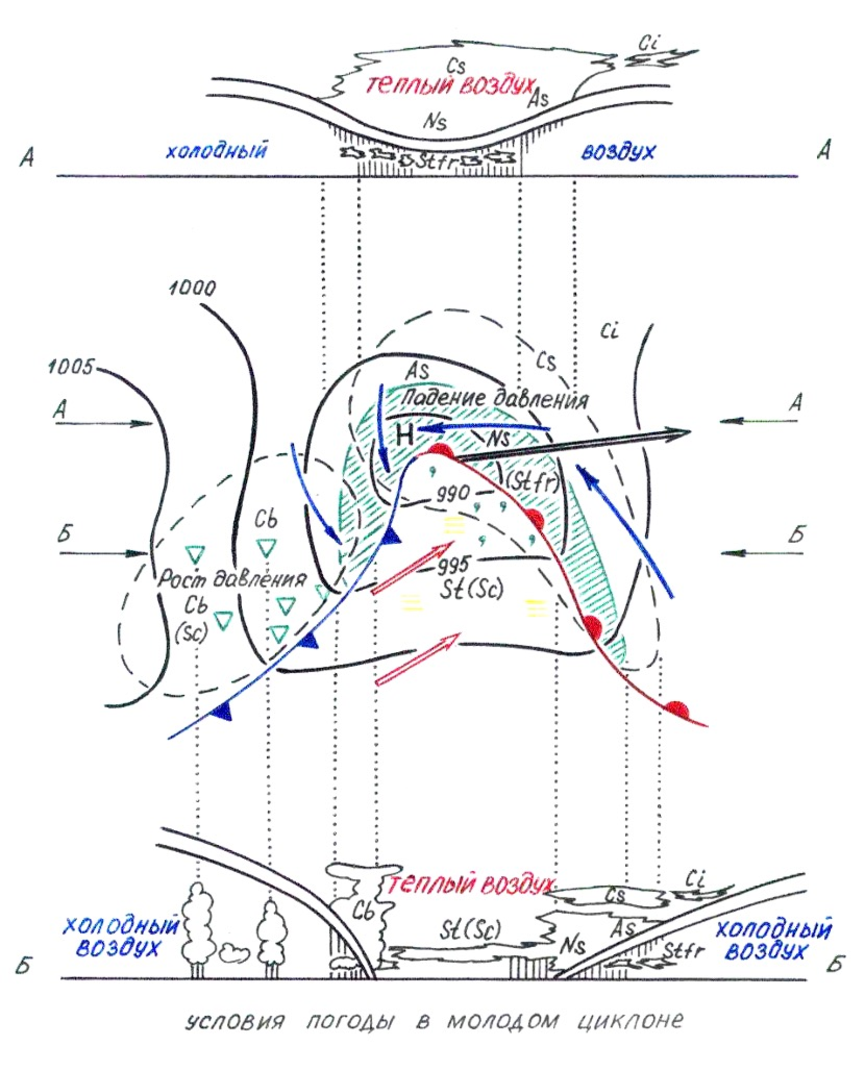
\includegraphics[scale=1.0]{03_cyclon.pdf}
   \caption{Молодой циклон}
   \label{fig:03_cyclon}
\end{figure*}


\textbf{Циклон}\index{циклон} \--- вихреобразное возмущение в
атмосфере с понижающимся давлением к центру. Характеризуется системой
ветров, дующих против часовой стрелки в северном полушарии и по
часовой стрелке в южном полушарии. Циклон зарождается, когда область
пониженного давления возникает на границе двух масс воздуха разной
температуры. В циклонах два фронта \--- холодный и теплый. Стадии
развития циклона: волна, волновой циклон, окклюзия или замыкание,
вихрь.

Стадия молодого циклона (рис.\ref{fig:03_cyclon}) характеризуется
наличием теплого сектора, т.е. сектора в южной части депрессии с
теплым воздухом и ограниченного спереди теплым фронтом, сзади \---
холодным. Холодный фронт в развивающемся циклоне движется быстрее
теплого. Стадия молодого циклона продолжается до тех пор, пока в
центре циклона у земной поверхности остается теплый
воздух. Продолжительность этой студии в среднем 12\otdo{}24~ч. В молодом
циклоне можно выделить три зоны, резко различающиеся по условиям
погоды.

\section{Антициклон}
\label{sec:anticyclon}

\begin{figure*}[htb]
   \centering
   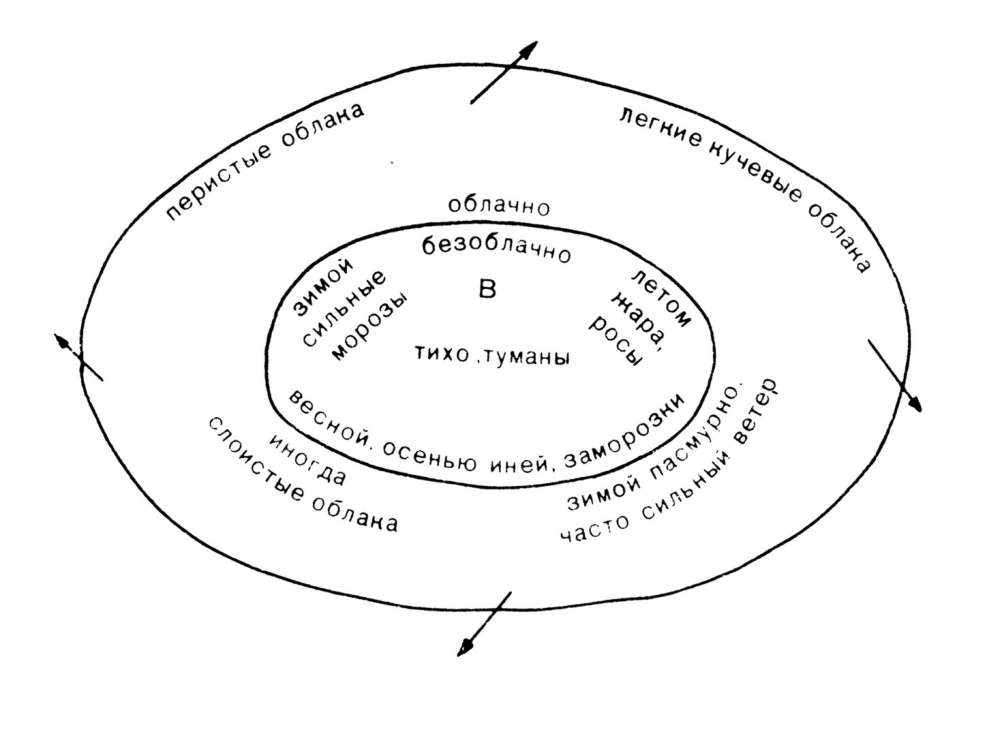
\includegraphics[scale=1.0]{04_anticyclon.pdf}
   \caption{Антициклон}
   \label{fig:04_anticyclon}
\end{figure*}

\textbf{Антициклон}\index{антициклон} \--- вихреобразное возмущение в
атмосфере с повышенным давлением в центре; область повышенного
атмосферного давления, состоящая из однородной воздушной массы
вращающейся по часовой стрелке в севером полушарии
(рис.\ref{fig:04_anticyclon} и против часовой стрелки в южном
полушарии.

\section{Атмосферный фронт}
\label{sec:front}

\textbf{Атмосферный фронт}\index{атмосферный фронт} \--- сравнительно
узкая (несколько километров) переходная зона между двумя воздушными
массами.

Если воздушный поток направлен от теплой воздушной массы к холодной,
то и фронт перемещается в этом направлении, такой фронт называется
\textbf{тёплым}\index{фронт!тёплый}.

\begin{figure*}[htb]
   \centering
   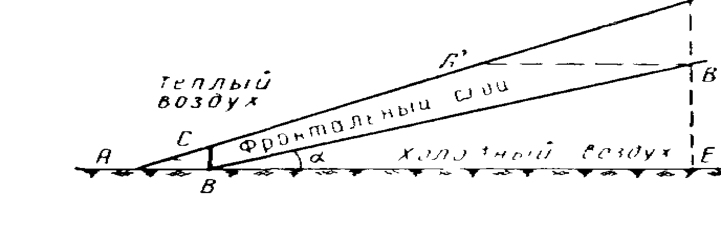
\includegraphics[scale=1.0]{05_vertical_front.pdf}
   \caption{Вертикальный разрез фронтального слоя}
   \label{fig:05_vertical_front}
\end{figure*}

Ширина фронтального слоя (рис.\ref{fig:05_vertical_front} в приводном
(приземном) слое (отрезок $AB$) наименьшая: от нескольких до десятков
километров, а на высоте 3\otdo{}5~км ($A'B'$) может достигать
300~км. В верхней половине тропосферы ширина фронтальной зоны может
быть еще больше. Вертикальная мощность слоя ($BC$ и $B'P$) обычно не
превышает 1~км. Горизонтальная проекция фронта $AE$ составляет
100\otdo{}1000~км, а его высота $EP$ \--- от 1 до 10~км.

Обычно толщиной фронтального слоя пренебрегают и считают, что фронт
\--- поверхность, которую называют фронтальной.

Различают следующие фронты: \textbf{основные}\index{фронт!основной}
(их называют тропосферными\index{фронт!тропосферный}, или
высокими\index{фронт!высокий}), \textbf{вторичные}\index{фронт!вторичный}
(приземные\index{фронт!призменый}, низкие\index{фронт!низкий}) и
\textbf{верхние}\index{фронт!верхний}.

Основными называются фронты, имеющие большую горизонтальную
(несколько тысяч километров) и вертикальную протяженность. Эти фронты
разделяют воздушные массы, существенно отличающиеся по своим
свойствам.

Скачок температуры при переходе через линию основного фронта на
приземной карте обычно превышает 5\grC.

Вторичными называются фронты небольшой горизонтальной протяженности,
(несколько сот километров).  Они разделяют различные порции одной и
той же воздушной массы. Высотная фронтальная зона со вторичными
фронтами не связана.

Верхними называются фронты, которые могут быть прослежены на картах
барической топографии, но не выявляются на приземных картах погоды.

Каждый основной фронт неоднороден по своим свойствам на всех
участках. Одни участки смещаются в сторону теплой воздушной массы,
другие \--— в сторону холодной, третьи \--- малоподвижны. Поэтому фронты
классифицируются по ряду дополнительных признаков.

Теплыми называются участки основного фронта, перемещающиеся в сторону
относительно холодной воздушной массы. За теплым фронтом
(рис.\ref{fig:06_warm_front}) перемещается теплая воздушная масса.

\begin{figure*}[htb]
   \centering
   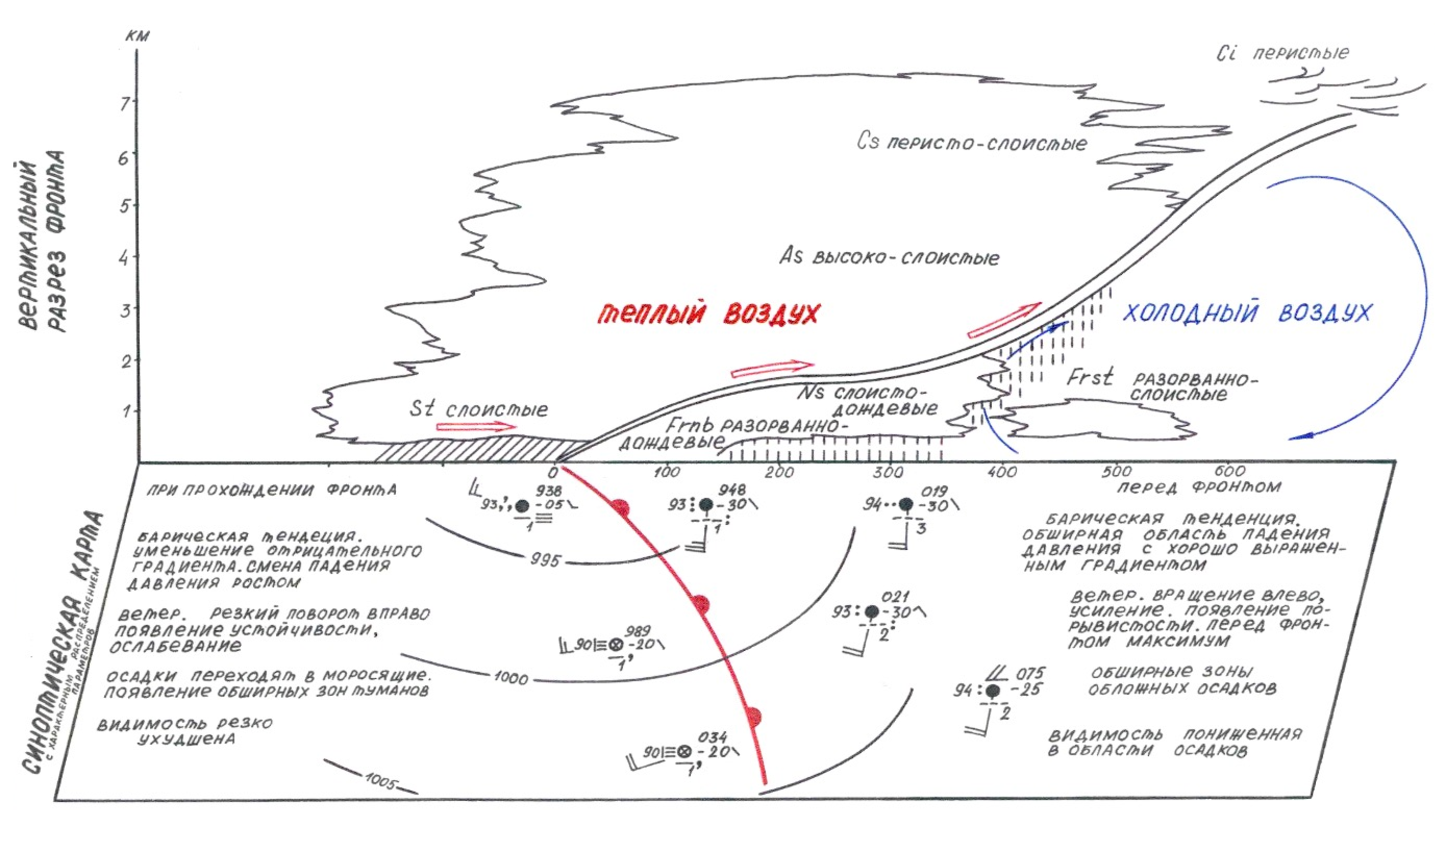
\includegraphics[scale=0.7]{06_warm_front.pdf}
   \caption{Тёплый фронт}
   \label{fig:06_warm_front}
\end{figure*}

\backmatter

\printindex

\end{document}
